%%%%%%%%%%%%%%%%%%%%%%%%%%%%%%%%%%%%%%%%%%%%%%%%%%%%%%%%%%%%%%%%%%%%%%%%%
%% Proposal Template created by Jessi Rick (jrick@uwyo.edu), Fall 2018 %%
%% Designed based on EG Mandeville's Dissertation Proposal %%%%%%%%%%%%%%
%% This is simply a recommendation to get you started-- feel free to %%%%
%% modify to whatever works best for you (and your advisor)! %%%%%%%%%%%%
%%%%%%%%%%%%%%%%%%%%%%%%%%%%%%%%%%%%%%%%%%%%%%%%%%%%%%%%%%%%%%%%%%%%%%%%%

%%%%%% Preamble of the document begins here %%%%%%
% mention the type of document, here we are using an article
\documentclass[letterpaper,12pt]{article}

% load the packages that we shall use for building the document
\usepackage[english]{babel}
\usepackage[utf8x]{inputenc}
\usepackage{natbib}
\usepackage{amsmath}
\usepackage{graphicx}
\usepackage[colorinlistoftodos]{todonotes}
\usepackage{subcaption}
\usepackage[margin=1in]{geometry} %% sets 1" margins
%\renewcommand{\baselinestretch}{1.5} %% this sets to 1.5 spacing
%\usepackage{setspace} %% these two set double spacing
%\doublespacing %% goes with previous

\bibpunct{(}{)}{;}{a}{}{,}  % this is a citation format command for natbib

% for fancy headers (testing)
\usepackage{fancyhdr}
\pagestyle{fancy}
\usepackage[font={small,sf},format=plain,labelfont={bf,up}]{caption}
\fancyhf{}
\fancyhead[l,lo]{YOUR NAME \textit{Dissertation Proposal}}
\fancyhead[r,ro]{\thepage}

% this package is for tables
\usepackage{booktabs}
% write the title and author here
% You must supply your own values
\title{Title of this proposal: Lots of work ahead}
\author{Your Name}
\date{Version: \today}

%%%%% Preamble to the document ends here %%%%%%

\begin{document}
\maketitle

% next we include the different sections. 
% Each section is included in the document
\section{Overview and Objectives}
Here you can provide general background information relevant to your project. This will serve as a general introduction/overview for your project. You can include references by using \texttt{\textbackslash cite\{citation\}} or \texttt{\textbackslash citep\{citation\}} or \texttt{\textbackslash citealt\{citation\}}, depending on how you want it formatted (like this: \cite{Cohen2016}; \citep{Cohen2016}; \citealt{Cohen2016}). If you have your bibliography connected, the possible citations will pop up as you start typing an author name 

More information about my project. My research seeks to answer the the following general questions:
\begin{enumerate}
    \item \textbf{QUESTION 1, related to chapter 1} \\
    Explanation of this question.
    
    \item \textbf{QUESTION 2, related to chapter 2} \\
    Explanation of the question

    \item \textbf{QUESTION 3, related to chapter 3} \\
    Explantion of the question.
    
\end{enumerate}
\section{Relevance and Justification}

Here is an explanation of why your project matters-- what impact will this research have?
%%%%%%%%%%%%%%%%%%%%
\section{Background}
%%%%%%%%%%%%%%%%%%%%

%%%%%%%%%%%%%%%%%%%%%%%%%%%%%%%%%%%%%%%%%%%%%%%%%%%%
\subsection{Topic 1 Heading}
%%%%%%%%%%%%%%%%%%%%%%%%%%%%%%%%%%%%%%%%%%%%%%%%%%%%
[background on this topic]

%%%%%%%%%%%%%%%%%%%%%%%%%%%%%%%%%%%%%%%
\subsection{Topic 2 Heading}
%%%%%%%%%%%%%%%%%%%%%%%%%%%%%%%%%%%%%%%
[background relevant to this topic]

%%%%%%%%%%%%%%%%%%%%%%%%%
\subsection{Study System}
%%%%%%%%%%%%%%%%%%%%%%%%%

%%%%%%%%%%%%%%%%%%%%%%%%
\subsubsection{One part of the study system}
%%%%%%%%%%%%%%%%%%%%%%%%
Here is some information about my study system

%%%%%%%%%%%%%%%%%%%%%%%%%%
\subsubsection{Another part of the study system}
%%%%%%%%%%%%%%%%%%%%%%%%%%

Here is some information about the specific fish that I study.

%%%%%%%%%%%%%%%%%%%%%%%%%%%%%
\subsection{Preliminary Work}
%%%%%%%%%%%%%%%%%%%%%%%%%%%%%

Here is an explanation of preliminary work that you have done-- have you already collected samples in the field? Do you have preliminary genetic/morphometric/etc. data? Include those things here. This might be somewhere you might include a table! Here's an example of that (Table \ref{table:species-location}).

Alternatively, preliminary work could be included as a subsection for each objective, depending on what makes the most sense for your project.

%Tables can be generated using tablesgenerator.com or truben.no
%This is a test of using the tables file. Here is an example table, which I can refer to as Table \ref{table:species-location}:

\begin{table}[ht]
\centering
\caption{This is the caption for this table}
\label{table:species-location}
\begin{tabular}{@{}lllll@{}}
\toprule
Location  & Species (Field ID) & Count & Feature3 & Feature4 \\ \midrule
Kigoma & Lates angustifrons  & 2   & Number   & number   \\
Kigoma & Lates microlepis  & 11   & Number   & number   \\
Kigoma & Lates mariae  & 5 & Number   & number   \\
Kigoma & Lates stappersii  & 38 & Number   & number   \\
Kigoma & Lates spp. unknown & 10 & Number & number \\
North Mahale & Lates angustifrons  & 0   & Number   & number   \\
North Mahale & Lates microlepis  & 0   & Number   & number   \\
North Mahale & Lates mariae  & 15   & Number   & number   \\
North Mahale & Lates stappersii  & 9   & Number   & number   \\
South Mahale & Lates angustifrons  & 0   & Number   & number   \\
South Mahale & Lates microlepis  & 0   & Number   & number   \\
South Mahale & Lates mariae  & 18  & Number   & number   \\
South Mahale & Lates stappersii  & 18   & Number   & number   \\ \bottomrule
Total & & 143 & &
\end{tabular}
\end{table}
\section{Research Plans}
\subsection{Objective 1: Heading for this chapter}
\label{objective1}
A brief bit of introduction to this chapter (1-2 paragraphs)

\subsubsection{Research Plan}
 What methods do you have planned for this chapter? Here you should describe what your concrete plans are for addressing this objective. You also might want to include a figure in this portion, such as Fig. \ref{fig:colonization_hypothesis}.
 
 %% FIGURE %%
\begin{figure}[tb]
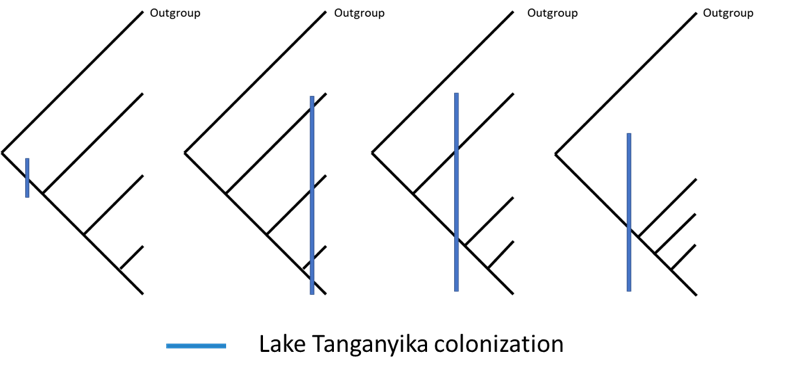
\includegraphics[width=\textwidth]
{figures/colonization_hypothesis.png}\caption{\label{fig:colonization_hypothesis} Hypotheses to test about the colonization of Lake Tanganyika (LT) by Lates fishes and their diversification times. (A) A common ancestor colonized LT and each of the species split off from the others in succession; (B) the four species diversified prior to colonizing LT; (C) two different ancestors colonized LT, followed by diversification of one of those species; (D) a common ancestor colonized the lake, and the four species split at roughly the same time, forming a true radiation.}
\end{figure}
%%%%
 
 \textsc{Method A ---} You can use subheadings to separate out different things you'll be doing for this chapter. Perhaps your subsections can be "sampling," "data generation," and "analysis" (these are what mine are!).
 
 \textsc{Method B ---} And here's a second subsection of things that I'll be doing.
 
\subsubsection{Specific Questions}
\begin{enumerate}
    \item \textbf{Question \#1}
    
    A bit of explanation about this question, if necessary, and perhaps what your hypothesis is for this question.
    
    \item \textbf{Question \#2}
    
    Explanation for this question.
    
\end{enumerate}

\subsubsection{Expected Outcomes}
What things do you anticipate coming from this chapter?
\subsection{Objective 2: Heading for this chapter}
\label{objective2}
A brief bit of introduction to this chapter (1-2 paragraphs)

\subsubsection{Research Plan}
 What methods do you have planned for this chapter? Here you should describe what your concrete plans are for addressing this objective.
 
 \textsc{Method A ---} You can use subheadings to separate out different things you'll be doing for this chapter. Perhaps your subsections can be "sampling," "data generation," and "analysis" (these are what mine are!).
 
 \textsc{Method B ---} And here's a second subsection of things that I'll be doing.
 
\subsubsection{Specific Questions}
\begin{enumerate}
    \item \textbf{Question \#1}
    
    A bit of explanation about this question, if necessary, and perhaps what your hypothesis is for this question.
    
    \item \textbf{Question \#2}
    
    Explanation for this question.
    
\end{enumerate}

\subsubsection{Expected Outcomes}
What things do you anticipate coming from this chapter?
\subsection{Objective 3: Heading for this chapter}
\label{objective3}
A brief bit of introduction to this chapter (1-2 paragraphs)

\subsubsection{Research Plan}
 What methods do you have planned for this chapter? Here you should describe what your concrete plans are for addressing this objective.
 
 \textsc{Method A ---} You can use subheadings to separate out different things you'll be doing for this chapter. Perhaps your subsections can be "sampling," "data generation," and "analysis" (these are what mine are!).
 
 \textsc{Method B ---} And here's a second subsection of things that I'll be doing.
 
\subsubsection{Specific Questions}
\begin{enumerate}
    \item \textbf{Question \#1}
    
    A bit of explanation about this question, if necessary, and perhaps what your hypothesis is for this question.
    
    \item \textbf{Question \#2}
    
    Explanation for this question.
    
\end{enumerate}

\subsubsection{Expected Outcomes}
What things do you anticipate coming from this chapter?
\section{Relationship to work in progress}
\subsection{Work by Others}
If there are others (i.e. collaborators) who are working on things relevant to your project, this is a good place to explain their research.

\subsection{Side projects}
\subsubsection*{Side project \#1}
Information about this project. This is a way of letting your committe know about projects that you're working on that may not directly relate to your planned thesis-- this also serves as a list of possible chapters that you could add in case one of the ones you propose doesn't work out!

\subsubsection*{Side project \#2}
Information about this project.
\section{Relationship to long-term goals}
This is a section that you can probably leave out, or include if you feel like you'd like to say something about how your project will get you to where you want to be-- it is often useful for your committee members to know where you want to end up, so that they can help to guide you in that direction (i.e. if you are using genomics as a tool, but aren't particularly interested in the methods, then perhaps they won't focus on asking you detailed questions about the methods).
\section{Timeline}
This can be a general explanation of what you are thinking of for a timeline for completing your project. It doesn't need to be too specific, but you should suggest the order of things, or planned fieldwork to collect samples, or timeline for generating genomic data, etc.

% special sections for tables and figures
% then go after the main text of the article
% you can also copy paste from these sections and codes there
%\include{tables}
%\include{figures}

% This part is for including references and citations
% you can change the bibliography style to whatever you'd like
\bibliographystyle{sysbio}

%% change to your own bibliography!
\bibliography{example}

% The document must end with this code
\end{document}